\newpage
\section{Auswertung}
\label{sec:Auswertung}

\subsection{Temperaturverläufe}
    Die Termperaturverläufe in einem Diagramm dargestellt:
    \begin{figure}
        \centering
        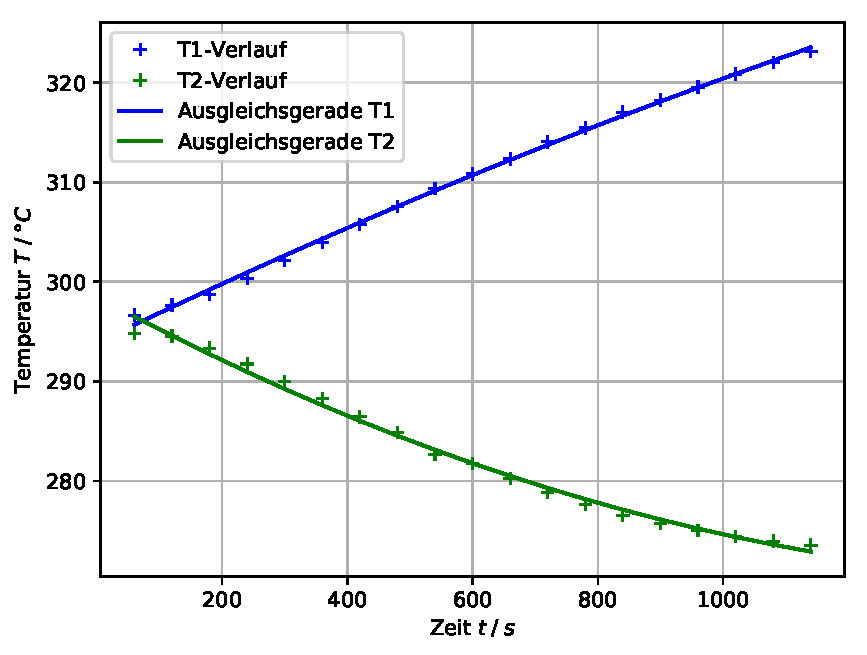
\includegraphics[width=\textwidth]{build/plot_temp.pdf}
        \caption{Temperaturverläufe}
        \label{fig:plot_temp}
\end{figure}

\subsection{nicht-lineare Ausgleichsrechnung}
    Mit der folgenden Näherung, werden nun die in \ref{fig:plot_temp}
    dargestellten Ausgleichsgeraden bestimmt\cite{curvefit}:
    \begin{equation}
        T(t)=At^2+Bt+C
        \label{eqn:ausgleichsgerade}
    \end{equation}
    \begin{table}
        \centering
        \begin{tabular}{c || c | c}
            \toprule
            & $T_1\;/\;K$ & $T_2\;/\;K$ \\
            \midrule
            A\;/\;$K/s^2$& -3,813E-06 & 1,007E-05 \\
            B\;/\;$K/s$& 0,030 & -0,034 \\
            C\;/\;$K$& 293,875 & 298,519 \\
            \bottomrule
        \end{tabular}
    \end{table}
\subsection{Differentialquotienten}
    Exemplarisch werden für vier Messwerte der Differentialquotienten $dT1/dt$ und
    $dT2/dt$ berechnet.
    Für die Näherung von \eqref{eqn:ausgleichsgerade} folgt somit:
    \begin{equation}
        \frac{dT}{dt}=2At+Bt
    \end{equation}
    
    \begin{table}
        \centering
        \begin{tabular}{c c c c}
            \toprule
            Zeit $T\;/\;s$ & $T_1$ & d$T_1$/d$t$ & Fehler\\
            \midrule
            240,0 & 300,35 & 0,029 & \\
            480,0 & 307,55 & 0,027 & \\
            840,0 & 317,045 & 0,024 & \\
            1080,0 & 322,045 & 0,022 & \\
            \midrule
            Mittelwert &&  0,025 & \\
            Standartabweichung &&   &\\
            Ungenauigkeit &&    &\\
            \bottomrule
        \end{tabular}
        \caption{Differentialquotienten für $T_1$}
        \label{fig:tab_T1t}
    \end{table}

    \begin{table}
        \centering
        \begin{tabular}{c c c c}
            \toprule
            Zeit $T\;/\;s$ & $T_2$ & d$T_2$/d$t$ & Fehler\\
            \midrule
            240.0 & 291.75 & -0.029 & \\
            480.0 & 284.85 & -0.024 & \\
            840.0 & 276.55 & -0.017 & \\
            1080.0 & 273.95 & -0.012 & \\
            \midrule
            Mittelwert &&  -0,021 & \\
            Standartabweichung &&   &\\
            Ungenauigkeit &&    &\\
            \bottomrule
        \end{tabular}
        \caption{Differentialquotienten für $T_2$}
        \label{fig:tab_T2t}
    \end{table}
    \newpage
    \subsection{Bestimmung der Güteziffer}
    Wie in Gleichung (4a!) dargestellt, lässt sich aus dem zuvor berechneten
    Differentialquotienten die Güteziffer [v] bestimmen.\\
    Die Wärmekapazität des Kupfers $m_k\;c_k$ wurde bereits in Abschnitt (hier!) erwähnt.
    Für die Wärmekapazität von Wasser $m_1\;c_w$ gilt \cite{wasser}:
    \begin{equation*}
        m_1\;c_w = 4190\frac{J}{kg\;K} 	\Rightarrow 12570\frac{J}{K}
    \end{equation*}

    \begin{table}
        \centering
        \begin{tabular}{c c c c}
        \toprule
        Zeit $t\;/\;s$ & Güteziffer !$v_{ideal}$ (nach Gl. 4'!) & Güteziffer !$v_{real}$ (nach Gl. 3b!) & Abweichung \% \\
        \midrule
        
        \end{tabular}
    \end{table}
    \subsection{Massendurchsatz}
    \subsection{Mechanische Kompressionsleistung}
    
